\documentclass[letterpaper]{article} % DO NOT CHANGE THIS
\usepackage{aaai2026}  % DO NOT CHANGE THIS
\usepackage{newtxtext}   % DO NOT CHANGE THIS
\usepackage{helvet}  % DO NOT CHANGE THIS
\usepackage{courier}  % DO NOT CHANGE THIS
\usepackage[hyphens]{url}  % DO NOT CHANGE THIS
\usepackage{graphicx} % DO NOT CHANGE THIS
\urlstyle{rm} % DO NOT CHANGE THIS
\def\UrlFont{\rm}  % DO NOT CHANGE THIS
\usepackage{natbib}  % DO NOT CHANGE THIS AND DO NOT ADD ANY OPTIONS TO IT
\usepackage{caption} % DO NOT CHANGE THIS AND DO NOT ADD ANY OPTIONS TO IT
\frenchspacing  % DO NOT CHANGE THIS
\setlength{\pdfpagewidth}{8.5in}  % DO NOT CHANGE THIS
\setlength{\pdfpageheight}{11in}  % DO NOT CHANGE THIS
%
% These are recommended to typeset algorithms but not required. See the subsubsection on algorithms. Remove them if you don't have algorithms in your paper.
\usepackage{algorithm}
\usepackage{algorithmic}

%
% These are are recommended to typeset listings but not required. See the subsubsection on listing. Remove this block if you don't have listings in your paper.
\usepackage{newfloat}
\usepackage{listings}

\usepackage[utf8]{inputenc}
\usepackage{booktabs}
\usepackage{amsmath}
\usepackage{amssymb}
\DeclareCaptionStyle{ruled}{labelfont=normalfont,labelsep=colon,strut=off} % DO NOT CHANGE THIS
\lstset{%
	basicstyle={\footnotesize\ttfamily},% footnotesize acceptable for monospace
	numbers=left,numberstyle=\footnotesize,xleftmargin=2em,% show line numbers, remove this entire line if you don't want the numbers.
	aboveskip=0pt,belowskip=0pt,%
	showstringspaces=false,tabsize=2,breaklines=true}
\floatstyle{ruled}
\newfloat{listing}{tb}{lst}{}
\floatname{listing}{Listing}


\setcounter{secnumdepth}{2} % Allow section numbering

\title{Comparing CSP Replanning, MDP Value Iteration, and Q-Learning\\
for Stochastic Grid Navigation}
\author{
    % Authors
    Milena Paques\textsuperscript{\rm 1},
    Wael Drif\textsuperscript{\rm 1},
    Rafael Palma Santos\textsuperscript{\rm 1}
    Komildzhon Samadov\textsuperscript{\rm 1}
}
\affiliations{
    % Affiliations
    \textsuperscript{\rm 1}Université Libre de Bruxelles\\
    milena.paques@ulb.be, wael.drif@ulb.be, rafael.palma.santos.da.silva.mendes@ulb.be, komildzhon.samadov@ulb.be
}

\begin{document}
\maketitle

\begin{abstract}
This project compares three AI approaches on the same stochastic path planning task: a constraint-based replanning method, a model-based Markov Decision Process (MDP) solver, and model-free Reinforcement Learning (RL). The shared environment is a grid world with static obstacles, hazardous cells, and stochastic motion. We evaluate success rate, return, and runtime across difficulty levels and grid sizes. Results show that MDP is the most robust under high uncertainty, CSP replanning is strong on easier instances but degrades sharply at higher difficulty, and tabular Q-learning performs well when uncertainty is moderate but can fail on hard sparse-reward cases.
\end{abstract}

\begin{links}
    \link{Code}{https://github.com/your-user/infoh410project}
\end{links}

\section{Problem Formulation}
The problem is a stochastic grid navigation task defined as follows:
\begin{itemize}
    \item \textbf{Environment Map.} The environment is an $N \times N$ grid where cells are identified by their row and column coordinates $(r,c)$ for $r, c \in \{0, \dots, N-1\}$. The grid contains a set of static obstacles $O$ (impassable cells) and a set of hazards $H$ (passable cells that incur an additional penalty).
    \item \textbf{Task.} An agent must navigate from a fixed start cell $s_0=(0,0)$ to a fixed goal cell $g=(N-1,N-1)$.
    \item \textbf{State space.} The state space $S$ consists of all non-obstacle cells: $S = \{(r,c) \mid 0 \le r < N, 0 \le c < N \} \setminus O$. A state is $s=(r,c)$, where $r$ is the row index and $c$ is the column index.
    \item \textbf{Action space.} $A=\{\text{Up},\text{Down},\text{Left},\text{Right}\}$.
    \item \textbf{Transitions.} Dynamics are stochastic. Let $p$ be the slip probability. When taking action $a$, the agent moves in the intended direction with probability $1-p$, and slips to one of the two orthogonal (lateral) directions with probability $p/2$ each. If a move (intended or slipped) points outside the grid boundaries or into an obstacle $O$, the agent simply remains in its current state.
    \item \textbf{Reward.}
\begin{equation}
R(s,a,s')=
\begin{cases}
+25, & \text{if } s'=g\\
-5, & \text{if } s'\in H\\
-1, & \text{otherwise}
\end{cases}
\end{equation}
This establishes a base step cost of $-1$, an additional penalty of $-4$ for terminating a step in a hazard cell ($H$), and a $+25$ reward for reaching the goal.
\end{itemize}
Episodes terminate immediately upon reaching the goal $g$ or after a maximum limit of $H_{\max}=4N$ steps. This problem supports: (1) deterministic feasibility planning with explicit constraints (ideal for CSP), (2) model-based stochastic planning with full transition probabilities (perfect for MDP), and (3) model-free learning from sampled interaction (suitable for RL).

\section{Methods}
\subsection{Approach A: CSP Replanning}
We model a deterministic plan as a sequence of state variables $(X_0, X_1, \dots, X_T)$ with domains $D_t \subseteq S$, subject to the following constraints:
\begin{equation}
X_0=s_{\text{current}},\; X_T=g,\; X_t \notin O,\; X_t \notin H,\; \text{Adj}(X_t, X_{t+1})
\end{equation}
where $s_{\text{current}}$ is the agent's current state, $O$ is the set of obstacles, $H$ is the set of hazards, and $\text{Adj}(X_t, X_{t+1})$ ensures that $X_{t+1}$ is a valid deterministic single-step orthogonal move from $X_t$. At each step, the agent solves for the shortest feasible trajectory to the goal that strictly avoids all obstacles and hazards. It executes the first action of this plan and immediately replans from the new state if a stochastic slip causes a deviation.

\subsection{Approach B: MDP Value Iteration}
We compute the optimal policy by solving the known MDP using value iteration. We iteratively update the state values $V_k(s)$:
\begin{equation}
V_{k+1}(s)=\max_{a\in A}\sum_{s'\in S} P(s'|s,a)\left[R(s,a,s')+\gamma V_k(s')\right]
\end{equation}
where $P(s'|s,a)$ is the exact transition probability model mapping the intended and slip dynamics, $R(s,a,s')$ is the reward function defined earlier, and $\gamma=0.95$ is the discount factor. The optimal policy is extracted greedily: $\pi^*(s)=\arg\max_{a\in A} Q^*(s,a)$.

\subsection{Approach C: RL Q-Learning}
We train a model-free tabular Q-learning agent that learns strictly from environment interaction via an $\epsilon$-greedy exploration strategy. The action-value function is updated after observing the reward $r$ and the next state $s'$:
\begin{equation}
Q(s,a) \leftarrow Q(s,a)+\alpha\left[r+\gamma\max_{a'\in A}Q(s',a')-Q(s,a)\right]
\end{equation}
We use a constant learning rate of $\alpha=0.2$, a discount factor of $\gamma=0.95$, and a linearly decaying exploration rate $\epsilon$ that drops from $1.0$ to $0.05$ over the course of training.

\section{Experimental Design}
The experiments were conducted on three main scenarios: Easy $(N=10, p=0.05, o=0.12, h=0.08)$, Medium $(N=12, p=0.15, o=0.18, h=0.10)$, Hard $(N=14, p=0.25, o=0.22, h=0.12)$, where $o$ is the density of obstacles and $h$ is the density of hazards.
For each scenario and method, we evaluate 120 episodes and record:
\begin{itemize}
\item success rate,
\item average return,
\item average steps on successful episodes,
\item total runtime (preparation plus evaluation).
\end{itemize}

Additional runs on $N\in\{8,10,12,14,16\}$ (80 episodes each) measure runtime growth and success stability (see Figure~\ref{fig:runtime}). Additionally, all random generators use fixed seeds. The repository provides a single command to regenerate all tables and figures.

\section{Results}
Table~\ref{tab:main} summarizes the three main scenarios.

\begin{table}[ht]
\centering
\small
\caption{Main scenario results.}
\label{tab:main}
\begin{tabular}{llrrr}
\toprule
Scenario & Method & Success & Return & Time(s) \\
\midrule
Easy & CSP & 1.0000 & 6.55 & 0.2562 \\
Easy & MDP & 1.0000 & 7.02 & 0.0322 \\
Easy & RL & 1.0000 & 6.79 & 0.1755 \\
Medium & CSP & 1.0000 & -1.44 & 0.4504 \\
Medium & MDP & 1.0000 & -0.01 & 0.0565 \\
Medium & RL & 1.0000 & -0.96 & 0.2336 \\
Hard & CSP & 0.1583 & -57.47 & 1.2358 \\
Hard & CSP (relaxed) & 0.9916 & -31.71 & 1.47 \\
Hard & MDP & 0.9833 & -24.48 & 0.3548 \\
Hard & RL & 0.0000 & -56.10 & 0.4086 \\
\bottomrule
\end{tabular}
\end{table}

\begin{figure}[ht]
\centering
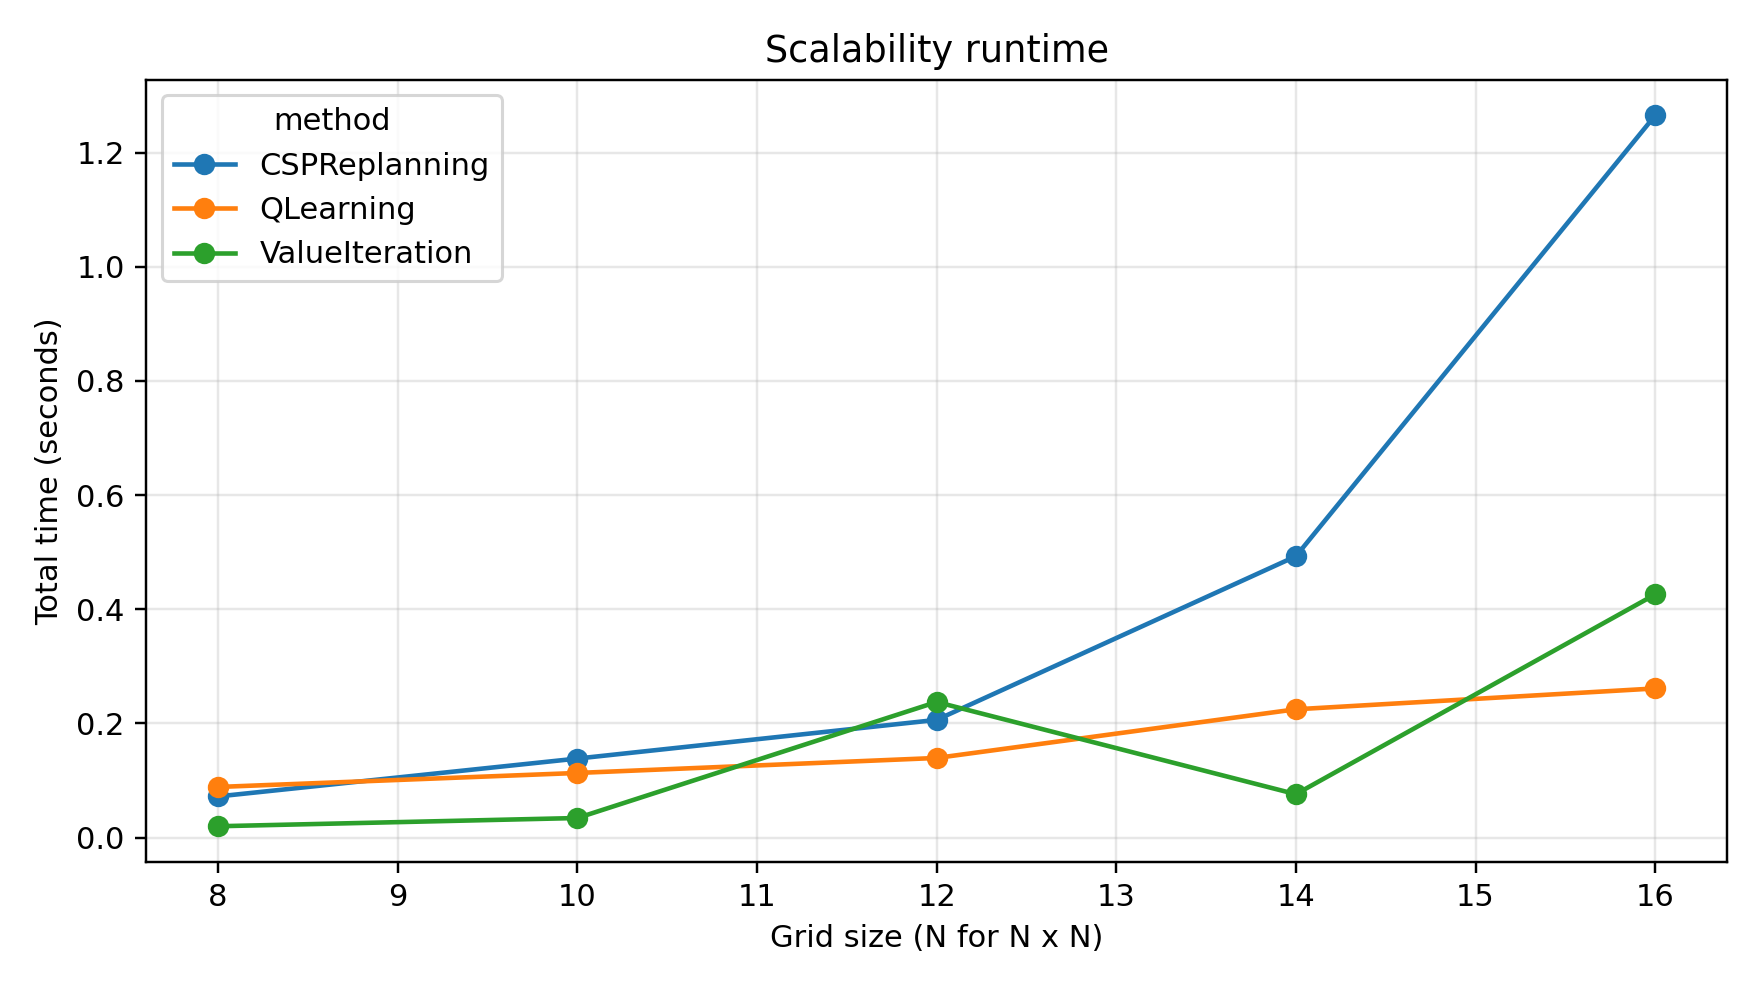
\includegraphics[width=0.95\columnwidth]{../results/scalability_runtime.png}
\caption{Scalability runtime versus grid size.}
\label{fig:runtime}
\end{figure}
strictly avoiding hazards for CSP makes it fail more often under high slip and dense hazards. However, introducing a second CSP that relaxes the hazard constraint if no path is found, restores navigability on the hard setting (boosting success to 0.9916), though at the cost of a lower average return (-31.71) compared to MDP and a longer runtime (1.47s).
The results show that MDP gives the strongest robustness under high stochasticity (hard success rate 0.9833). CSP replanning is competitive on easy and medium settings, but it fails more often under high slip and dense hazards. RL reaches strong performance on easy and medium settings, but the hard setting shows that finite tabular training can be insufficient in sparse-reward, high-uncertainty conditions.

\section{Qualitative Comparison}Relaxing these safety constraints restores feasibility but leads to sub-optimal paths that accumulate hazard penalties. 
\textbf{CSP replanning} has the strength of transparent constraints and direct control over safety rules. However, it proves brittle when uncertainty causes frequent replanning or when strict hazard avoidance removes many feasible trajectories. In contrast, \textbf{MDP value iteration} explicitly optimizes the expected long-term return under stochastic transitions, providing strong robustness. Its main drawback is the requirement for a full transition and reward model, alongside a computational cost that grows directly with the state space size. Finally, \textbf{Q-learning} offers the advantage of requiring no prior model, allowing it to adapt purely from interaction. On the downside, it is highly sensitive to the exploration schedule and training budget, and its tabular representation scales poorly as the environment grows.

\textbf{When to use what.}
In summary, one should use CSP when safety constraints are strict and dynamics are mostly predictable. MDP is preferable when a reliable environment model is available and handling uncertainty optimally is critical. RL remains the method of choice when prior model knowledge is unavailable and online adaptation is required.

\section{Technical Quality and Reproducibility}
The codebase is modular (environment, methods, evaluation, runner), deterministic via fixed seeds, and fully reproducible from command line.

\section{Conclusion}
Across identical tasks, MDP planning is the best overall trade-off in this project, especially on the hard stochastic setting. CSP replanning is fast to implement and interpretable but less robust at higher uncertainty. Q-learning is promising but needs more sample-efficient function approximation for difficult settings.

\bibliography{references}

\end{document}
